% UPDATED BY MARCUS SCHAGERBERG, 2023
% CREATED BY WOLFGANG AHRENDT, 2021

% WRITTEN BY MARTIN BLOM, 2023
This section will discuss the results of the project. This encompasses examining any unreached goals and presenting the performance evaluation of the tool. Later on the user testing and it's impact will be discussed, as well as the development process it self and any possible future improvements.

% WRITTEN BY JAKOB WINDT, 2023
\section{Performance Evaluation}
    In section \ref{performance-benchmark}, we displayed a table showcasing some performance statistics of the simulation software. The benchmark summarizes the current expected performance of the simulation. The test was completed using the script, mentioned in section \ref{performance-method}, to determine the FPS with a varying amount of vehicles that are simulated in the Masthugget build. Additionally, the same test was performed in both quality mode, meaning realistic physics modeling for each vehicle, and performance mode, with a much simpler physics engine. The results showcase the overall benefit of running the simulation in performance mode, but also how there is a need to further improve the performance to simulate more expansive road systems.

% WRITTEN BY JAKOB WINDT & MARCUS SCHAGERBERG, 2023
\section{Delimitations}
    As mentioned throughout the report, some delimitations were set for the project. These limitations included a built-in editor, height maps and driver behaviors. Currently, the only way to edit the map of the simulation is to use Unity. This means that the road network can only be modified in development mode, which is not available for the users.

    Even though the simulation is displayed in 3D, the roads can only be placed on flat surfaces. This means that there are no tunnels or bridges in the simulation, which would have been needed if an area included, for example, mountains or rivers. Adding height to the simulation would have been a difficult task to implement due to the lack of available accurate real world height map data.

    Lastly, another question that might arise is whether a randomness factor needs to be implemented in order for the simulation to be realistic, such as different driver behaviours like aggressiveness or navigation errors. This is not something that has been added as it is not a requirement for a realistic simulation. These behaviours operate on a micro level, whereas congestion or traffic flows are on a macro level. The traffic flows in the road system are formed over time in a larger scope, where the individual behaviours or driver randomness factors are not as prevalent. Existing tools, such as PTV Visum, are often built on models where individual agents are not simulated at all, as mentioned in section \ref{traffic-simulations}.

% WRITTEN BY MARCUS SCHAGERBERG, 2023
\section{Ethical aspects}
    As mentioned in section \ref{ethics}, it is important to consider the ethical implications of creating an accessible tool. For regular citizens, even if they could use this tool to find improvements to road systems, they are unable to execute them in practice as they do not have the financial assets, knowledge or equipment to construct roads. However, the users could potentially use the tool to influence others with that possibility. Therefore, a comprehensive end user license agreement would need to be compiled, in combination with clear information about what the software is meant to provide, and what it should not be used for. Section \ref{ethics} also points out the need to state any assumptions or model biases in an accessible manner which would need to be included. Rigorous testing would have to be performed to validate the correctness of the simulation and statistics, comparing the tool to existing tools as well as real world data.


% WRITTEN BY MARCUS SCHAGERBERG, 2023
\section{Unreached Goals}
    Some features took more resources and longer time to implement than initially estimated, which limited development in other areas. The most significant example of this is the road creation system. When defining the goals and planning the project, an asset called RoadArchitect had been found that supported this\cite{road-architect}. The asset was well-known and had an extensive documentation. However, when starting the development using this asset, several severe bugs were identified. We think the issue is that it was developed for an earlier release of Unity, and was not compatible with our version even though there was no documentation of this. RoadArchitect supported creation of roads and intersections with many features, such as traffic lights, road markings, railings and bridges. This was a major setback as we had to develop our own road creation tool. Adding all the needed features to the road creation tool was an extensive process that would have been avoided if we could use RoadArchitect as it had nearly all the features needed for this project.

    An area which was less prioritised due to the time constraints was the support for public transport, which was only added with basic support. The goal was to have a working public transportation system, with the ability to change a parameter in the simulation for how much of the traffic is handled through it. This would allow users to find the optimal balance between public transport and cars.

    A map editor was supposed to be developed to allow users to create their own maps and road systems to analyse. The time and change in priorities did not allow for the time to add this. This is definitely something that would need to be added in the future if the tool would be released. As of now, it is only possible to edit the maps in the built-in Unity Editor, which is not available when generating an executable version of the tool.

\section{User Testing Feedback}
    Receiving feedback on the project was very valuable. However, we were limited to only one iteration of user testing due to time restraints and project scope, which limited our ability to refine and adapt the simulation based on the feedback received. Having additional rounds of user testing, ideally with the same users, would have been highly beneficial. This would allow us to observe how users adapt to the software over time and evaluate any implemented changes made in response to their feedback.
    
    % WRITTEN BY FELIX JÖNSSON, 2023
    \subsection{Evaluation of the software}
        According to the user feedback, we found our tool to be intuitive and easy to use, regardless of the users' prior background. The control scheme, although not clearly communicated in every different state of the simulation, was deemed intuitive and straightforward.  Every tester made requests for additional features, but felt that the ones currently implemented were easy to grasp and could be utilized easily by the tester through the minimalistic UI. The generic testers requested more immersive enhancing details, such as rear-view mirrors when sitting inside the car, have the steering-wheel turn in synchronicity with the movement of the vehicle, and add further details to the environment. This feedback would be valuable for future development, but was not prioritized in the scope of this project due to time constraints. The overall impression was that the simulation, as it stands now, has a lot of good features but would need to focus on extending these while maintaining the user-friendly approach to be able to compete with other simulators.
    
    % WRITTEN BY MARCUS SCHAGERBERG, 2023
    \subsection{Changes made based on the user testing feedback}
        In order to eliminate the ambiguity between the two statistics related buttons, it was decided to remove one of them and instead dynamically change the content based on the context. It was changed so that if the statistics panel is open while a vehicle is selected, it displays the individual statistics related to that vehicle. Otherwise, it displays the overall statistics for the entire road network. This solution was proposed to the tester and the response was that it would be suitable solution.

        As some users felt that it was a bit cumbersome to navigate around, the camera controls were changed so that the keyboard is used for movement around the plane, and the mouse to rotate the camera. This change made the tool in line with most games, as well as other software, such as CAD programs. This improves the accessibility and intuitiveness as users can recognise the controls from previous experiences. The movement speed was also changed to depend on the zoom level, so that the camera moves slower when zoomed in on vehicles or intersections, while being faster when positioned at a higher altitude. This allows the user to quickly move between areas of the network, while still being able to have fine control over the movement when zoomed in.

        A button was also added to toggle the colour coding feature that can colour the roads based on current statistics, such as congestion levels or emissions. As illustrated in \ref{fig:color-roads}, this feature is useful for visualising the current performance of the road network and swiftly identifying problematic areas when observing the system from a macro perspective. In response to feedback from the generic testers, we also added an additional control scheme that allows camera movement using the arrow keys.
        
    \begin{figure}[H]
        \begin{tabular}{cc}
            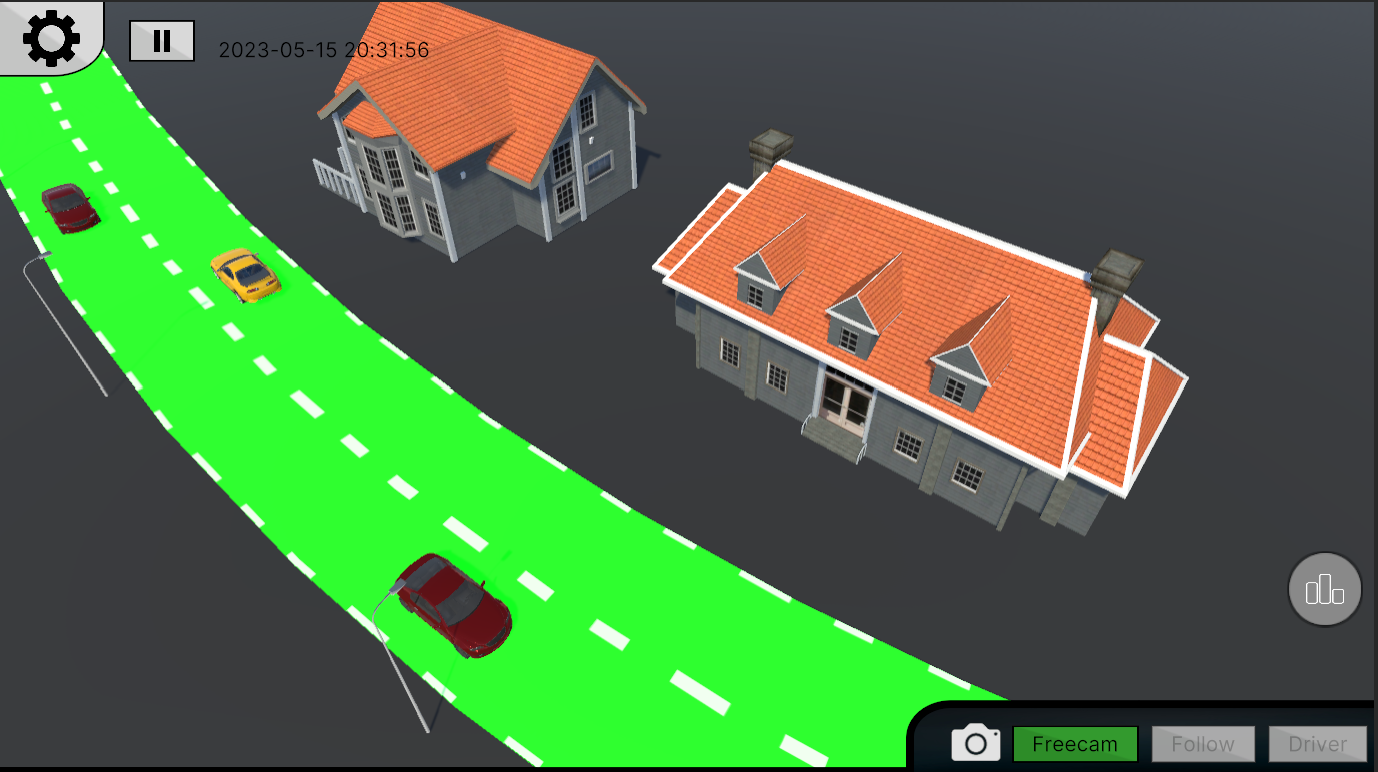
\includegraphics[width=0.48\linewidth]{Project_report/figures/method/green road.png} & 
            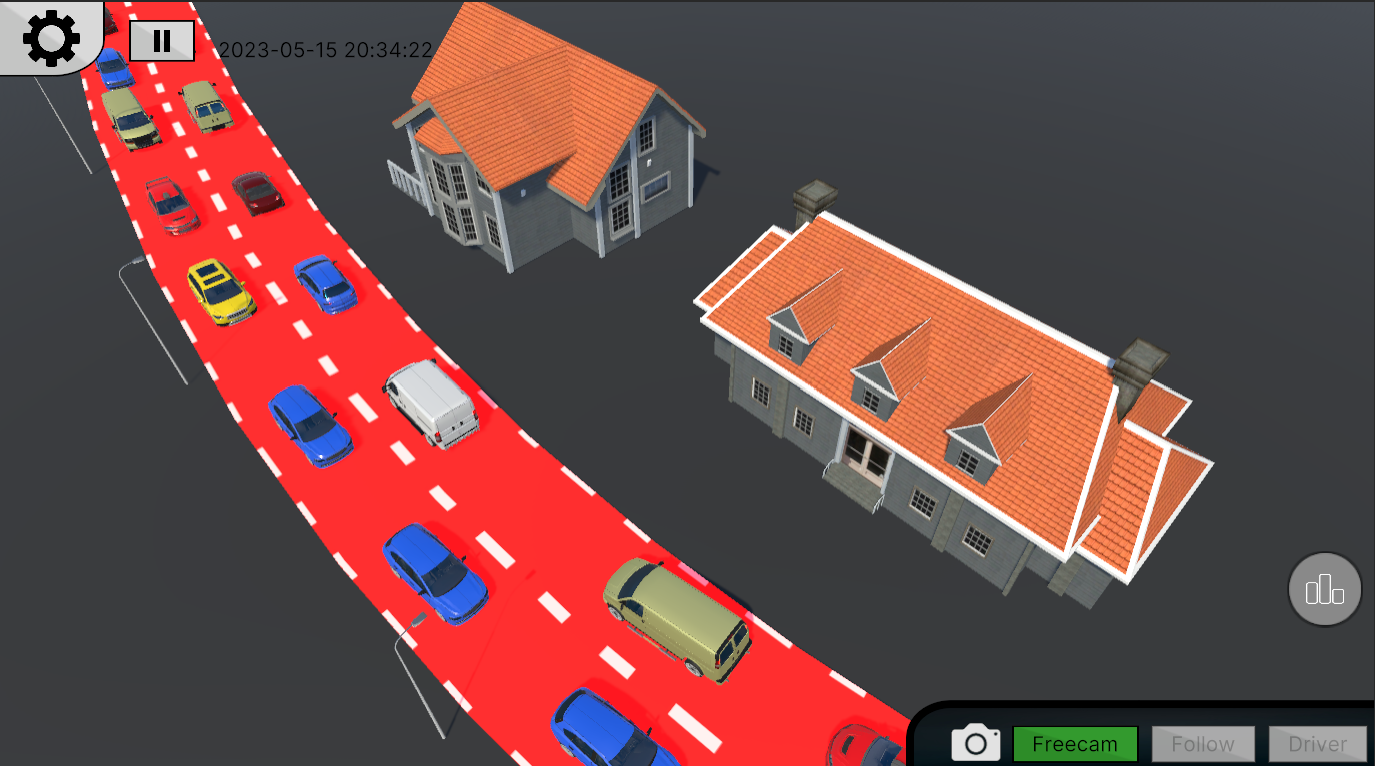
\includegraphics[width=0.48\linewidth]{Project_report/figures/method/red road.png} \\
        \end{tabular}
        \caption{Colored road based on current fuel consumption}
        \label{fig:color-roads}
    \end{figure}
    
    
% WRITTEN BY JAKOB WINDT, 2023
\section{Development Process}
    As previously mentioned in section \ref{sub:weekly-sprints}, the decision was made to follow the scrum framework. This allowed the group to set clear goals for each week, which simplified the process of dividing work. For the most part, this worked as well as expected. However, something that was noticed during the project was that the backlog was slowly increasing with tickets. Each week, a small number of tickets were delayed for different reasons, which was the cause of the problem. 

    During the development of the simulation, code reviewing was an important factor in making sure the code was correct, commented, and well written. This worked well for the majority of the time, but minor problems arose for larger pull requests. The reason behind this is due to the problem that when someone tries to merge an extensive amount of code at the same time, the time and effort required by the code reviewer increases. This is because the reviewer first has to try and understand the logic and functionality of the code itself. Therefore, if a code reviewer is tasked with reviewing a large pull request, the reviewer might not have the same attention to detail compared to when reviewing less code, resulting in a worse review.

    % WRITTEN BY MARTIN BLOM, 2023
\section{Future Improvements}
    This section will present any future improvements or changes that we would like to implement. We will partly provide motivations as to why these improvements were not made, and if unclear, why we deem them important. Improvements without any explanation as to why they are missing can be presumed to be a result of lack of time.
    
    % WRITTEN BY JAKOB WINDT, 2023
    \subsection{Road and Intersection Types}
        When designing large road networks, especially outside cities, highways are critical. Highways are currently not supported in the simulation because of a few different reasons. To begin, there is functionality for multiple lanes when creating roads within the built-in Unity road generator. However, the vehicles are not able to switch lanes in the simulation, making multiple lanes unusable. Since lane switching isn't supported, vehicles do not have the ability to overtake each other. There are also no highway entrances or exits in the simulation, which would need to be implemented for highways to function correctly.

        For intersections, the simulation only supports three and four way intersections. These intersections can be created with either one-way or regular two lane roads, or a mix of both. In reality, there are other intersection types such as the roundabout that there currently is no support for. For this to be implemented in the future, the yielding of the cars has to improve from their current state.

        % WRITTEN BY MARCUS SCHAGERBERG, 2023
        Expanding the support for different types of road signs and traffic rules would also be an improvement over other tools that in most cases does not support this. An example of this is how our tool supports the priority to the right rule, which could mean that in certain situations an intersection could be easily congested due to vehicles on one of the roads always having to yield to those on the other. Additional signs such as those defining rules for parkings could also affect the simulation, making certain parking spaces restricted for example during certain times of day or for non-residents. Due to the nature of the tool being low level with simulation of individual vehicles, there is room for improvement with features like these which would separate the tool even more on the market, creating a unique feature set.

    % WRITTEN BY JAKOB WINDT, 2023
    \subsection{OSM}
        In the current state of the simulation, OSM imports are supported but flexible enough to be fully usable. Currently, OSM datasets can be imported in the pre-build of the simulation. This means that to replicate a real-life location in the simulation, the user would have to manually import the OSM file into the Unity project, and then change the path to the file within the code. In the future, there should be functionality to either import OSM data directly from within the simulation, or a way to import OSM files without having to manually edit code.
        
        Additionally, OSM imports are not perfect in its current stage. Because of the lack of support for intersection types, the road network can end up generating in an unfinished state. In the same way, there have been other issues, for example, when two intersections are located next to each other. One of them usually fails to generate due to the overlap between the intersections. Finally, not all data from the OSM file is used when generating the world. In addition to the current POIs outlined in \ref{poi}, one data point that should be implemented in the future, are charging stations for electric vehicles.

    % WRITTEN BY JAKOB WINDT, 2023
    \subsection{Vehicle Types}
        With the previously mentioned charging and fuel stations, different vehicle types representing electric and gas driven cars could be included. This would improve the statistical accuracy of the simulation, allowing the user to modify the differential between the two types. The reason this should be implemented is because of the increase in electric vehicles registered in the world, and their effect on emissions\cite{IEA}. 
        
        Equally important, other forms of transport should be included as well. These would include trains, trams, and taxis. With the inclusion of these vehicles, the amount of cars in a road network should decrease due to the use of public transport. However, this depends on the efficiency, availability, and cost of said public transport. With the reduced amount of cars in the road network, both efficiency will increase, and total emissions should decrease.

    % WRITTEN BY MARCUS SCHAGERBERG, 2023
    \subsection{Performance Optimisation}
        One of the major limitations of the tool is the performance. Simulating individual agents is a performance intensive task. The physics engine used by the vehicles to provide realistic handling uses a lot of resources, especially when simulating many vehicles. The performance mode helps with this, but would need to be developed further to allow larger networks to be simulated with reasonable performance. The mathematical calculations it currently uses could be optimized or perhaps even simplified while still fulfilling the requirements.

        A great way of achieving a significant increase in performance is by multithreading heavy workloads. Nowadays almost all computer processors have multiple threads allowing them to perform tasks in parallell. Some workloads are more difficult to parallellize, as multiple cores simultaneously reading and writing from the same memory locations can interfere with each other. A heavy task that could easily benefit from multithreading is the OSM import, where there is a clear separation between several import stages. This would allow the maps to be generated quicker, especially on less powerful hardware. It is also possible to multithread the vehicle physics calculations, however this is much harder as they interact with each other. Therefore, all vehicles need to be updated before the program can move on, which will limit the benefit of this optimisation.


    % WRITTEN BY MARCUS SCHAGERBERG, 2023
    \subsection{Simulation Improvements}
        One of the areas where there is a lot of potential for improvement is related to the simulation itself. The simulation could be made more realistic by improving the target assignment algorithm, which determines where the vehicles should navigate to. The algorithm can be expanded to include parameters such as the time of day, to determine what the vehicles should do. This would allow the implementations of rules causing many vehicles to simultaneously drive from houses to companies and industrial areas in the morning, and then returning in the evening. This would further stress the road system and is something to take into consideration.
        
        In addition to the buses following routes and stopping at the bus stops, their behaviour could be extended to follow schedules with a limited pool of available buses. This would limit the amount of people that could use the public transport system, causing more vehicles to appear in the network. Expanding on the public transport integration is something that could make the tool even more useful and is an innovative area, as noted during the user tests where it was mentioned that other tools lack this feature. This could be used for finding the optimal balance between public transport and personal vehicles, and aid in transportation planning.

    % WRITTEN BY MARTIN BLOM, 2023
    \subsection{Statistics}
        Statistics is one of the areas where improvements can almost always be made when analysing data. Therefore, many new ways of visualizing the same data can put fourth to widen the target audience. Moreover, with the extensive amounts of data that can be produced, many different comparisons can be made. The currently implemented statistics and graphs are related to important environmental factors like fuel-consumption and emissions, as well as network performance related statistics such as congestion over time. With the multitude of different techniques of representing data, including new parameters, the possibility of adding more statistics is almost endless.

        Statistics could also be improved visually, by adding filters or features that highlight or better indicate the data that the user is searching for. An example would be adding more visual highlighters - in the same fashion that the the roads are highlighted in red when congested - for other variables such as road surface wear.

    % WRITTEN BY MARTIN BLOM, 2023
    \subsection{Map Editor}
        An area where the tool is lacking, is the creation of the network. As it stands, the only way to manipulate the environment is through the built-in Unity editor. This creates a barrier for users without any knowledge of Unity, and might discourage them from further usage of the tool. Even with the understanding of how to do this, it is a tedious and time consuming process. Having to use a separate software for some tasks also not intuitive for the user. To solve this, a built-in map editor would need to be developed, allowing the user to move, manipulate, create and delete any of the aforementioned aspects inside the tool. This would dramatically improve both the efficiency and the simplicity of the process, further boosting the tool's user-friendliness.